\section{Analisi dei requisiti}

% Esporre brevemente i requisiti a cui il sistema proposto deve rispondere.
% Concentrare l'attenzione sugli aspetti più rilevanti, facendo eventualmente uso di opportuni diagrammi di alto livello.

% Vincoli circa la lunghezza della sezione (escluse didascalie, tabelle, testo nelle immagini, schemi):
% Numero minimo di battute per 2 componenti: 6000
% Numero massimo di battute per 2 componenti: 8000

Per questo progetto, l'obiettivo di massima è la realizzazione di un sistema impiegabile in un ambiente indoor di tipo universitario (in particolare, una biblioteca dotata di aule studio),
monitorando il numero di persone stimato per stanza per tutto il periodo di funzionamento del sistema attraverso l'intercettazione di pacchetti WiFi.

Un servizio di monitoraggio dell'affollamento di ambienti indoor consiste in una serie di sensori distribuiti nelle stanze dell'edificio che registrano le presenze;
poiché si assume essere un luogo pubblico, il sistema deve poter monitorare l'ambiente senza dipendere dalla collaborazione attiva da parte dell'utente.

Il servizio deve essere facilmente fruibile e non deve invasivo né per l'edificio né per l'infrastruttura di rete esistente.
I sensori possono dunque essere più o meno complessi compatibilimente con le esigenze dell'ambiente di installazione.

Infine, dai casi riportati in letteratura si può dedurre che il problema della privacy nella gestione dei dati è di fondamentale importanza e va considerato assolutamente.

\subsection{Raccolta dei requisiti}

Per poter condurre un lavoro efficace, si è deciso in inziare dalla scelta di un ambiente reale e di effettuarne l'analisi, eventualmente con la collaborazione della struttura stessa.

Come ambiente di riferimento, si è deciso di considerare la Biblioteca Centrale Roberto Ruffilli del Campus di Forlì.
Esso è un ambiente indoor strutturato su due piani e 18 stanze adibite ad aule studio.

Dialogando con il personale e con alcuni studenti, si è manifestato l'interesse ad un sistema semplice ed immediato in grado di dare visivamente informazioni sul numero di persone;
sembra sia necessario che l'eventuale sistema non sia invasivo, né per quanto riguarda l'installazione dell'hardware, né per quanto riguarda l'eventuale software necessario per la sua fruizione.
Per quanto non sia fondamentale, il personale della libreria ha mostrato interesse verso la possibilità di avere alcuni statistici oltre al conteggio attuale, purché siano dati liberamente pubblicabili e nel pieno rispetto della privacy sui dati.

\subsection{Requisti funzionali}\label{subsec:req:func}

Dall'analisi delle informazioni raccolte, sono state identificate le seguenti entità che interagiscono per il corretto funzionamento del sistema:

\begin{description}
    \item[Servizio di raccolta dati]
      tramite sensori per l'individuazione della presenza e il conteggio dei device studiati;
    \item[Servizio di visualizzazione dell'affollamento]
      per permettere l'accesso alle misure in tempo reale, sia da parte degli studenti che dello staff;
      può essere interessante suddividere i dati visualizzati in:
      \begin{itemize}
        \item informazioni sui dati raccolti per uno specifico edificio;
        \item informazioni globali al sistema;
      \end{itemize}
    \item[Servizio di visualizzazione degli statistici]
      per permettere allo staff e a chiunque sia interessato di accedere a informazioni anonime e generali
      derivabili dai dati raccolti per il funzionamento del sistema.
\end{description}

Di seguito in \Cref{fig:use-cases} una rappresentazione tramite UML dei casi d'uso individuati.

\begin{figure}[H]
  \centering
  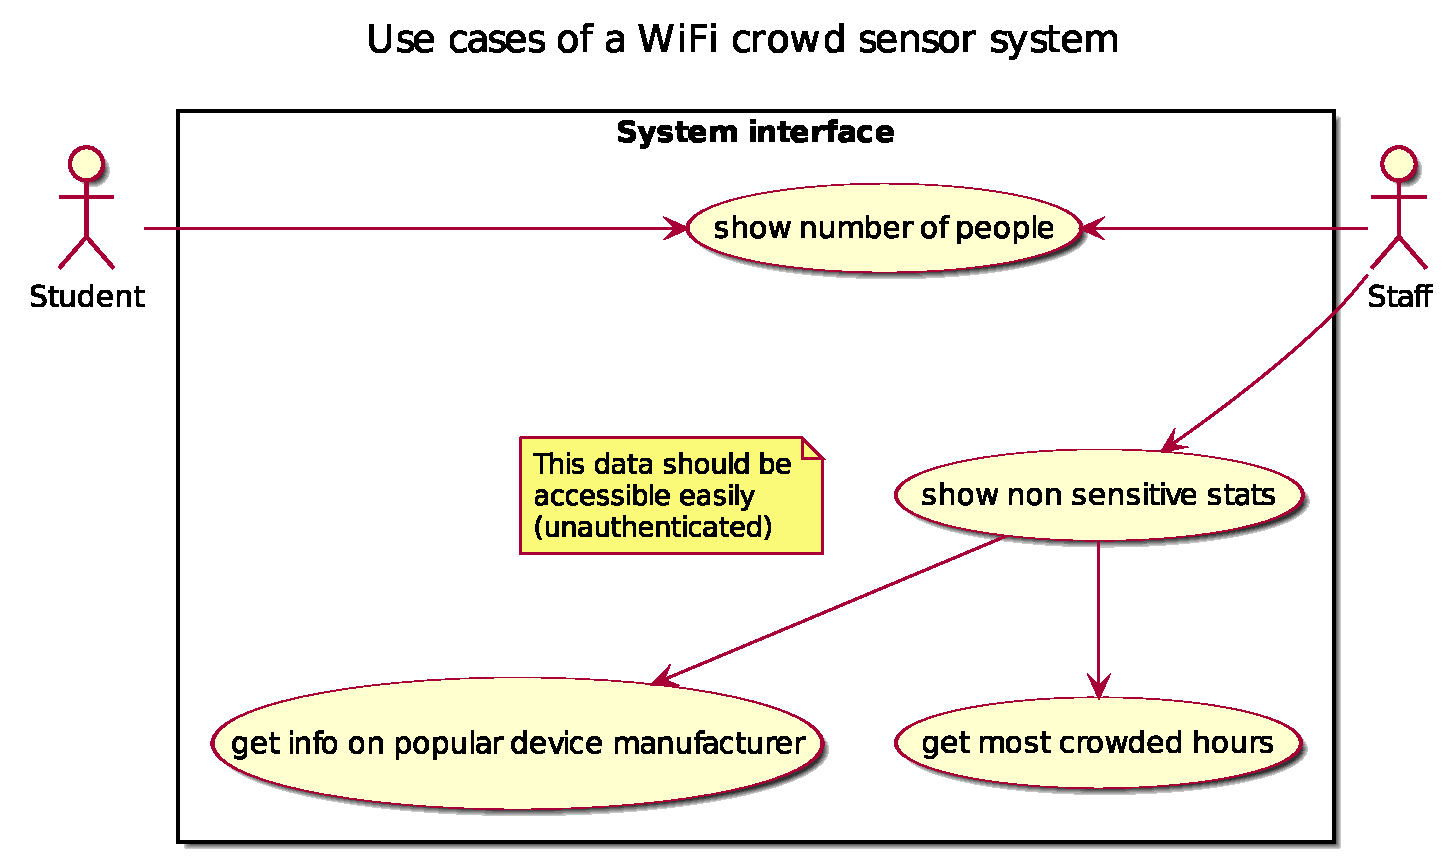
\includegraphics[width=\textwidth]{res/out/use-case.eps}
  \caption{Diagramma UML che riassme i casi d'uso del sistema}%
  \label{fig:use-cases}
\end{figure}

\subsubsection{Servizio di raccolta dati}

Il funzionamento del sistema prevede l'installazione non invasiva di sensori all'interno della struttura, presumibilmente uno per stanza;
tali sensori devono poter misurare il numero di persone all'interno delle stanze senza richiedere un contributo attivo da parte di ciascun individuo.

Un esempio può essere l'impiego di microcontrollori e/o SBC (\emph{Single Board Computer}) a basso consumo equipaggiati con un modulo WiFi in grado di lavorare in modalità promiscua.

\subsubsection{Servizio di visualizzazione dell'affollamento}

La misura dell'affollamento è il dato principale che il sistema deve raccogliere e fornire all'utente;
tale dato deve essere liberamente accessibile senza richiedere la registrazione dell'utente.
Inoltre, l'interfaccia di visualizzazione deve essere fruibile su quante più piattaforme possibile.

Tra i dati da visualizzare, è necessario mostrare:

\begin{itemize}
  \item un contatore del numero di dispositivi;
  \item un grafico rappresentante la variazione nel numero di persone nell'ultimo periodo (ad esempio, nell'ultima ora).
\end{itemize}

\subsubsection{Servizio di visualizzazione degli statistici}

Nella raccolta dei dati per il conteggio degli individui, vengono ottenute informazioni aggiuntive che possono essere considerate interessanti;
ad esempio, interecettando i pacchetti WiFi contenenti l'indirizzo MAC di ciascun dispositivo, è possibile registrare la popolarità dei vari vendor di dispositivi dotati di WiFi.

\subsection{Requisiti non funzionali}

In aggiunta ai requisiti elencati nella \Cref{subsec:req:func}, ne sono stati individuati altri di natura tecnlogica/implementativa:

\begin{description}
  \item[Semplicità di utilizzo]
    Il sistema deve risultare il quanto più possibile semplice ed intuitivo nell'utilizzo per la maggior parte degli utenti;
    ciò significa semplificare per quanto possibile le procedure per accedere alle funzionalità del sistema (ad esempio, realizzando un interfaccia web pubblicamente accessibile).
  \item[Architettura distribuita]
    Il sistema deve essere pensato per poter scalare da un ambiente ristretto composto da un singolo edificio con singola stanza ad una struttura più estesa composta da più edifici e/o più stanze;
    di conseguenza, affidarsi ad un'architettura monolitca sarebbe decisamente complicato e inefficiente.

    Per riuscire a garantire un corretto ed efficace funzionamento del sistema, occorre prendere in considerazione un'architettura distribuita e le conseguenti problematiche:

    \begin{description}
      \item[Consistenza]
        Il sistema deve riuscire a mantenere lo stato il più possibile consistente tra le repliche per supportare il carico di lavoro.
      \item[Scalabilità]
        Il sistema deve riuscire a gestire in maniera ottimale il carico a cui sottoposto.
      \item[Efficienza]
        Il sistema deve riuscire a rispondere a tutte le richieste senza tralasciarne alcuna.
    \end{description}
  \item[Privacy]
    Anche considerando le problematiche legali segnalate nella \Cref{sec:state-of-art}, la corretta anonimizzazione dei dati deve essere presa in considerazione.
  \item[Sicurezza]
    Per quanto pubblicamente \emph{consultabile}, il sistema deve permettere l'inserimento dei dati solo alle componenti autorizzate del sistema.
    In condizioni normali, non deve essere possibile per un utente umano modificare i contenuti raccolti;
    in casi eccezionali, il manutentore dovrebbe agire manualmente tramite API e con un token di autenticazione richiedibile per l'occasione.
  \item[Ingombro dei sensori e autonomia]
    Poiché il sistema non deve richiedere un'installazione invasiva, i sensori e i server locali devono essere:
    \begin{itemize}
      \item sufficientemente piccoli da poter essere nascosti in mobili già presenti nei locali senza modificazioni fisiche dell'ambiente;
      \item alimentabili in modo ``flessibile'' da batterie o da prese a muro.
    \end{itemize}
\end{description}
